%----------------------------------------------------------------------------------------

\documentclass[paper=a4, fontsize=11pt]{scrartcl} % A4 paper and 11pt font size

\usepackage[T1]{fontenc} % Use 8-bit encoding that has 256 glyphs
%\usepackage{fourier} % Use the Adobe Utopia font for the document - comment this line to return to the LaTeX default
\usepackage[english]{babel} % English language/hyphenation
\usepackage{amsmath,amsfonts,amsthm} % Math packages
\usepackage{mathtools}
\usepackage{lipsum} % Used for inserting dummy 'Lorem ipsum' text into the template
\usepackage[margin=2.8cm]{geometry}
\usepackage{xcolor}
\usepackage{listings}
\lstset{language=C++,
                basicstyle=\ttfamily,
                keywordstyle=\color{blue}\ttfamily,
                stringstyle=\color{red}\ttfamily,
                commentstyle=\color{green}\ttfamily,
                morecomment=[l][\color{magenta}]{\#}
}
\usepackage{mdframed}
\usepackage{graphicx}

\usepackage{sectsty} % Allows customizing section commands
\allsectionsfont{\centering \normalfont\scshape} % Make all sections centered, the default font and small caps

\usepackage{fancyhdr} % Custom headers and footers
\pagestyle{fancyplain} % Makes all pages in the document conform to the custom headers and footers
\fancyhead{} % No page header - if you want one, create it in the same way as the footers below
\fancyfoot[L]{} % Empty left footer
\fancyfoot[C]{} % Empty center footer
\fancyfoot[R]{\thepage} % Page numbering for right footer
\renewcommand{\headrulewidth}{0pt} % Remove header underlines
\renewcommand{\footrulewidth}{0pt} % Remove footer underlines
\setlength{\headheight}{15.0pt} % Customize the height of the header

\numberwithin{equation}{section} % Number equations within sections (i.e. 1.1, 1.2, 2.1, 2.2 instead of 1, 2, 3, 4)
\numberwithin{figure}{section} % Number figures within sections (i.e. 1.1, 1.2, 2.1, 2.2 instead of 1, 2, 3, 4)
\numberwithin{table}{section} % Number tables within sections (i.e. 1.1, 1.2, 2.1, 2.2 instead of 1, 2, 3, 4)

\setlength\parindent{20pt} % Removes all indentation from paragraphs - comment this line for an assignment with lots of text

%----------------------------------------------------------------------------------------
%	TITLE SECTION
%----------------------------------------------------------------------------------------

\newcommand{\horrule}[1]{\rule{\linewidth}{#1}} % Create horizontal rule command with 1 argument of height

\title{	
\normalfont \normalsize 
\textsc{Department Of Computer Science, University of Bath} \\ [5pt] % Your university, school and/or department name(s)
\horrule{0.7pt} \\[0.2cm] % Thin top horizontal rule
\Huge Inverse Kinematics Coursework \\ % The assignment title
\vspace{7 mm}
\Large CM50244 \: Computer animation and games I \\
\horrule{0.7pt} \\[0.0cm] % Thick bottom horizontal rule
}
\author{Garoe Dorta Perez, Dave Hibbitts, Ieva Kazlauskaite, Richard Shaw \\ \Large Unit Leader: Prof Phil Willis \\}  % Your name\\ 

\begin{document}
\vspace*{\fill}
\begin{center}
\begin{minipage}{1.0\textwidth}

\clearpage\maketitle % Print the title
\thispagestyle{empty}

\end{minipage}
\end{center}
\vfill
\clearpage
\setcounter{page}{1}

\section{Introduction and Objective}

\begin{center}
\begin{figure}
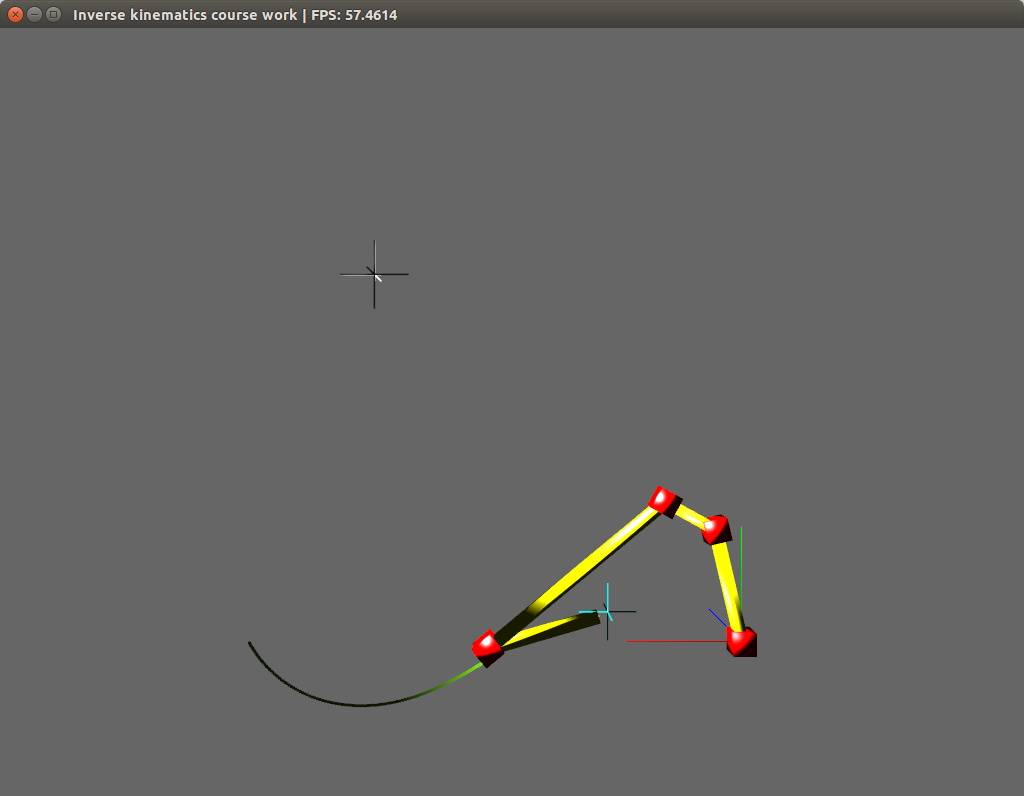
\includegraphics[scale=0.4]{chain3Dexample}
\caption{Final three dimensional simulation with the trace and a star showing the goal position.}
\end{figure}
\end{center}
 
In this project we explore the application of inverse kinematics in three-dimensional space. First, we construct a simple composite object which contains long rigid parts that are connected so as to allow flexibility of movement. The joints connecting the rigid rods are restricted and can either rotate in plane and act like simple hinges. Second, the method of inverse kinematics is explored in order to determine the configuration of the object, i.e. the relevant angles of the joints, when the object is given a task. The method works by planning the motion towards a goal, which is a point in three-dimensional space subject to constraints. Finally, the movement of the object is animated, and a number of non-physical (?) parameters are adjusted to deliver a visually appealing performance. \\

This report provides a brief account of the objectives of the project and the methods that were explored. Moreover, the issues that were encountered are discussed including problems concerning both the computations and the implementation. We discuss the implementation in Matlab and the computational method that we use for inverse kinematics. We proceed by explaining the operations and execution in OpenGL. The last section of this report includes a review of the performance and the limitations of the method, as well as a discussion of possible further improvements.


%------------------------------------------------

\section{Related Work}
What People do?

%------------------------------------------------

\section{Procedure}
In this section we discuss our approach to solving the problem at hand. We started by considering the corresponding two-dimensional situation where a planar object with a predetermined number of links is reaching towards a point in the plane. Our first attempt at a solution was to use forward kinematics where at each time-step we calculated the subsequent position using the current state and the desired position of the end-point. The first implementation was done in Matlab as we wanted to ensure that the method works as desired before exporting it to the OpenGL framework. In the meantime, we started working on the basic structure in OpenGL, for instance we drew the necessary primitives, such as triangles, squares and lines in two-dimensions, and proceeded by including some appropriate data structures and some primitive user interface. \\

The next step was to apply inverse kinematics in the case of our two-dimensional problem. We chose to use the Inverse Jacobian technique and implemented the method with both full inverse of the Jacobian matrix as well as the pseudoinverse. The motion of the object was displayed graphically, and we altered the number of limbs in order to test the performance of our method. At this stage the method still had a number of shortcomings even though it was restricted to motion in a plane. Firstly, the motion was not stable when the object was reaching towards a point that was outside the circular region. Secondly, the method favoured the movement of certain limbs without us explicitly specifying the constraints. We also improved the OpenGL user interface by adding mouse capture, and added chain class with bones and joints. In both Matlab and OpenGL the system is described using relative angles, i.e. starting at the origin, each subsequent angle is defined in the coordinate system of the previous one (picture???). \\

The main questions we faced at this point had to do with local behaviour of each joint and the numerical method used to solve the optimisation problem. The movement of the first few joints (those closest to the origin) appeared significantly more restricted than the movement of the end joints. To solve this issue, we normalise to get global behaviour of the whole system as opposed to local behaviour of each joint. In addition, the simulation naturally slows down as it gets very close to the destination due to the nature of the numerical method which tends to oscillate around the minimum point. This behaviour can be advantageous (especially in robotics) as it results in slow-down motion as it gets close to reaching the goal (e.g. grabbing an object or touching a surface) so as to avoid a severe collision. \\

We also note that the motion of the system is task-dependent, hence favouring the movement of a number of selected joints is reasonable. For example, if we assume that the object we are modelling is an arm, and the motion is defined as the arm reaching for a nearby object, it is logical to assume that the rotation of the elbow joint will be favoured against the rotation of the shoulder joint, etc. Therefore, we introduce a weight vector that is used to control the importance of the motion of each joint, and added constrains on the angles.\\

We continued to work on the graphical implementation and improved it in a number of ways. The simulation and rendering were separated into two different threads so that the speed of rendering does not affect the speed of the simulation. What is more, we started displaying the trace left by the tip of the object which makes it easier to track the motion of the object and adds visual appeal. \\

At this stage the Matlab and the OpenGL implementations were still independent, so we started importing the numerical method from Matlab to OpenGL. The resulting model was two-dimensional, used inverse kinematics, could be adapted to any number of limbs/joints, and had a simple user interface. \\

Naturally, the next step was to transform the model to the three-dimensional space. We first adapted the graphical framework to three dimensions, i.e. we could rotate the camera, and place a target anywhere in the space, however the object and the motion were still confined to a plane. \\

Let us now consider the implementation in both Matlab and OpenGL in more detail. The following two sections give a detailed account of the issues encountered during the implementation process, the solution methods we employed and the explanation of why we chose to use the particular approaches. \\


\subsection{Start with Matlab}
    \begin{enumerate}
    \item Issues
    \item How we solve them?
    \item Why we use what we use? (e.g. Inverse Jacobian)
  \end{enumerate}
\subsection{ Port the code to C++, OpenGL}
Our software was built on top of OpenGL version 4.3 so we can adopt the shaders introduced after 3.3 version, which uses a flexible pipeline. The following libraries are employed: GLFW for window managing, GLM  for including the matrix operations and matrix-vector data types, Boost provides smart pointers (which simplify memory management), GLEW which efficiently check which OpenGL extensions are supported on the platform that is used. The C++11 standard is used as it introduces better default thread and mutex libraries as well as other improvements. \\

First, we consider all the necessary conversions that let us display the three-dimensional world on a two-dimensional screen surface. Initially we have the \(z\) value set to zero, and hence worked in a two-dimensional space. In our world model each object has it's own model transformation matrix M. We also have a camera matrix that defines the camera position and orientation. Lastly, a projection matrix describes the mapping of a pinhole camera which plots the three-dimensional world onto a two-dimensional screen. For every object in the scene, pixel/screen coordinates \([u, v, 1]\) are defined by multiplying the vertices of each object by the Model-View-Projection (MVP) transformation matrix which gives the position of each pixel on the screen, i.e. transformed vertex = MVP *  object vertex. \\

\begin{mdframed}
\begin{scriptsize}
\begin{lstlisting}
//Renderer MVP calculation
viewProjection = projection * view;
//Calculate Model View Projection matrix
glm::mat4 MVP = viewProjection * modelMat;
\end{lstlisting}
\end{scriptsize}
\end{mdframed}

In the first version of our software, we would create all the OpenGL buffers for each object on each frame and destroy them at the end of each frame, which was inefficient. The problem was fixed by preallocating buffer objects (that store unformatted memory on the GPU) for each object at the start of the simulation, and then binding the framework to allocated storage (setting as the active), rendering and unbinding. \\

Next, we set up the necessary objects for rendering. We create a vertex object class that encapsulated the buffer objects used by OpenGL. The vertex specification is performed using the Vertex Array Object (VAO), and each vertex object has its own VAO attribute. For the two-dimensional model we adopt a simple shader program without lighting and we specify the colour directly. The actual implementation uses a vertex buffer object (VBO) for vertices so that each object has only the vertices listed sequentially in the corresponding buffer, and we have a colour buffer (CBO) of an identical size that contains the corresponding colours. The element buffer object (EBO) contains indices to a given vertex; it allows us to avoid replication of vertices and draw more efficiently. In particular, to define any rectangle (quad) that is a combination of two triangles, we only need to specify four vertices instead of using all six. \\

The initial implementation consisted of lines, squares and triangles, and an orthographic projection was used to represent the objects in two dimensions. To gain insight into the performance of our model, we included a frames per second counter which indicates how fast the scene is being rendered. In order to draw an objects, we implemented a \texttt{Drawable} class. All the objects that need to be displayed have to implement an interface defined by the \texttt{drawable} class and possess a function called \texttt{draw}. The window draws drawable objects and does not distinguish between them. The line, square and triangle are all subclass of the VertexObject class which itself is a subclass of Drawable. At this point we added the chain of rectangles and lines where lines represented bones and rectangles were joints. A \(4 \times 4\) rotation and translation matrices were introduced, so for each joint and at each time step the following calculation is performed:  \(\prod_{i=0}^I R_i T_i\) where \(R_i\) stands for the rotation of the joint and \(T_i\) corresponds to the translation of each bone. \\

\begin{mdframed}
\begin{scriptsize}
\begin{lstlisting}
class VertexObject: public Drawable {
	<...>
protected:
	//Model matrix
	glm::mat4 modelMat;
	//Model vertex related data
	std::vector<glm::vec3> vertices, normals, colors;
	std::vector<unsigned int> indices;
	glm::vec3 centroid;

	//Common object and buffers needed for OpenGL rendering
	GLuint vao, vbo, nbo, ebo, cbo;
};
\end{lstlisting}
\end{scriptsize}
\end{mdframed}

\begin{mdframed}
\begin{scriptsize}
\begin{lstlisting}
//Common draw call for all VertexObjects
void VertexObject::draw(Renderer& renderer) const {
	// Bind VAO and Buffers as the active ones.
	glBindVertexArray(vao);

	//Enable vertex buffer
	glEnableVertexAttribArray(0);
	glBindBuffer( GL_ARRAY_BUFFER, vbo);
	glVertexAttribPointer(0, 3, GL_FLOAT, GL_FALSE, 0, (void*) 0);
	
	//Enable the other buffers 
	<...>
		
	//Draw count objects of mode type
	glDrawElements(primitivePar.getMode(), primitivePar.getCount(),
	GL_UNSIGNED_INT, (void*) 0);
	
}
\end{lstlisting}
\end{scriptsize}
\end{mdframed}

In order to achieve a fluent and efficient rendering, we made the simulation process independent of rendering. Simulation and rendering are performed on two different threads, and have to access a shared resource concurrently. The synchronisation of these two processes is encapsulated in simulation controller class which uses a mutual exclusion lock variable. The rendering process has access to all the chain data while the simulation only uses the angles and lengths (taken from the copy of the chain) to perform the numerical calculations which advance the motion in time. The simulation runs almost continuously, it stops only to allow the renderer to look up the angle values each time it finishes rendering. This synchronisation mechanism allows the simulation and the rendering to perform their respective tasks as quickly as possible without any data corruption. \\

For visual appeal, we draw a trail that follows the chain tip. A circular array is used for efficient rendering; a fixed buffer is allocated on the GPU at the beginning of the simulation and we are tracking the movement of the tip of the chain. Each time the tip moves a sufficient (predetermined) amount, we record the current position and include it in the circular array. Once we run out of space, we return to the start of the array and replace the first value with the new one. Then the rendering is performed sequentially with all remaining values unchanged until we again reach the end of the array. This let's us make only small uploads of data to he GPU. \\

At this stage we added the simulation code originally developed in Matlab to our the two-dimensional model. To allow user input, we draw a triangle which could be moved using the mouse, and was used to mark the goal position. The mouse position was transformed using an inverse orthogonal projection. \\

One of the problems we faced had to do with the simulation thread accessing the rendering state, causing the software to fail if the frame rate was high (e.g. on the NVIDIA card). The problem was solved by allowing the simulation to access only the simulation data. Here we also used data encapsulation; a new class, called ChainModel, was created that only had the simulation data. The Chain class is a subclass of the ChainModel and with added attributes and methods for rendering purposes. The same applies to bone and joint classes. \\

\begin{mdframed}
\begin{scriptsize}
\begin{lstlisting}
//Simulation controller thread synchronization		
void SimulationController::executeSimulationLoop() {
	while (simulating) {
		lock.lock();
		simSolver.solveForStep(goal, stepSize);
		lock.unlock();
		std::this_thread::sleep_for(sleepTime);
	}
}

void SimulationController::updateChain() {
	lock.lock();
	simSolver.updateChain();
	lock.unlock();
}
\end{lstlisting}
\end{scriptsize}
\end{mdframed}

The simulation thread is in a loop either simulating or waiting for a new goal. It also checks when it's close to the goal and it stops at a given threshold, so update Jacobian loop is not called though the simulation thread is still running. The user can input a new goal position at any time, as the simulation loop will then solve for the new goal using the current chain state.\\

Our final improvement involved adapting the simulation and the display to work in a three-dimensional case. We construct the chain using rectangular parallelepipeds, while the shaders implemented a Gouraud shading algorithm. First, we added normal vectors to each vertex in every object; they point outwards from every vertices that is on the surface of the object, and for the vertices which are on the edges we use the mean of the neighbouring planar normals. Local illumination model combines the ambient, diffuse and specular light to give the colour intensities of the reflections, and the final shading is achieved by interpolating the vertices and normals. \\
\begin{center}
\begin{figure}[h]
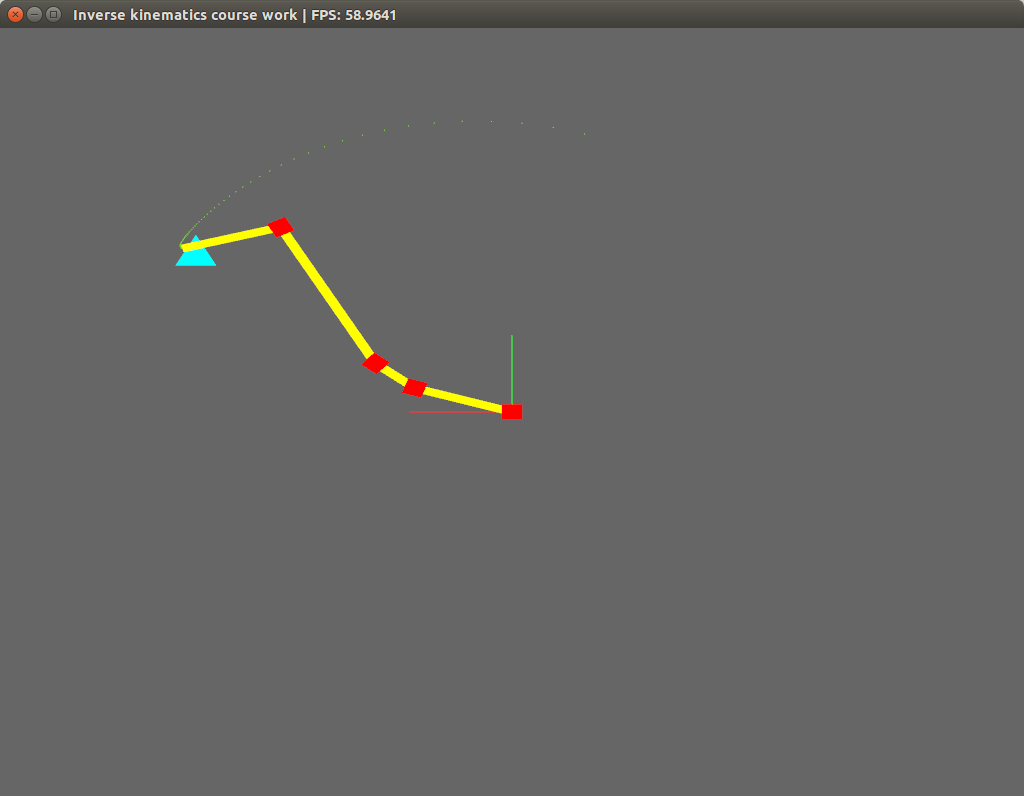
\includegraphics[scale=0.4]{chain2Dv2}
\caption{Final two dimensional simulation with the trace and a triangle showing the goal position.}
\end{figure}
\end{center}

In addition, we included keyboard input control. In the final version the user is able to control the camera angle by moving the mouse, and change the distance from the camera to the scene using the keyboard. In particular, we use the mouse to change the angle of the camera with respect to the \texttt{lookAtVector} and use the keyboard to move the camera position in a direction related to the \texttt{lookAtVector}, forward, backwards or side movements. The goal is moved using the camera position update (while right-clicking), where we update the position in the direction of the camera \texttt{lookAtVector}.\\

At this stage the model was displayed in three dimensions but was still confined to moving in the plane. We added a second rotation angle resulting in a rotation with respect to the \(z\)-axis followed by a rotation with respect to the \(y\)-axis, i.e. \( \mathbf{R}_z \mathbf{R}_y \mathbf{T}\). The resulting solver is fully three-dimensional. \\

\begin{mdframed}
\begin{scriptsize}
\begin{lstlisting}
//Update total transformation with current joint rotation and translation
currentMat = currentMat * glm::rotate(joints[i].getZRotAngle(), zAxis)
		* glm::rotate(joints[i].getYRotAngle(), yAxis)
		* glm::translate(glm::vec3(bones[i].getLength(), 0, 0));
\end{lstlisting}
\end{scriptsize}
\end{mdframed}

Final, a maximum number of simulation steps was specified to ensure that the simulation was not wasting CPU in case the goal was unreachable. Also, while the model is waiting for a new goal, the simulation thread is stopped, and once a point goal is added, it goes back to simulating. We had to artificially increase the time in the simulation (now it performs a simulation step and then waits for 20 ms), because otherwise the time step had to be decreased to \(10^{-6}\) which resulted in order to achieved a normal motion. Sleep time makes the computational load smaller on the CPU (i.e. we achieve the same accuracy with a lesser load on the CPU). 
  
\subsection{Exploration}
The following properties are to be explored.\\

1. Some way of indicating where the remote end of the linkage should move to in 3-space.\\
We have explored this already, see procedures section.\\

2. A way to change the physical properties such as rate at which the joints can change and the slow-out and slow-in of the movement of the end of the linkage as it leaves it current position and approaches the target position respectively.\\
We explored the possibilities in matlab, and, if time permits, we would implement it in c++.\\


3. Whether to model and thereby vary the flexibility of the rods.
We explored the possibilities in matlab, and, if time permits, we would implement it in c++.\\


%------------------------------------------------

\subsection{Summary and Conclusion}

\begin{enumerate}
\item Give a short summary of the project.
\item What the final thing would look like if we had more time to work on it?

\begin{itemize}
	\item Load 3D mesh objects and textures instead of parallelepiped...
	\item Add a better shading model
	\item Add a GUI
\end{itemize}
\end{enumerate}
%----------------------------------------------------------------------------------------

\end{document}